\chapter{Complex Attosecond Transient-absorption Spectroscopy}
\label{chap:CATS}

\section{Introduction}
\label{sec:intro_cats}

As seen in Chapter \ref{chap:ATS}, a rich amount of information can be extracted from ATS experiments.  Specifically, dynamics such as light-induced states and strong-field ionization excited states induced by a dressing field can be deduced from the change in photoabsorption.  However, these experiments are limited by the fact that they only have access to the imaginary part of the complex refractive index of the medium of interest. There should also be a corresponding changing in the real part of the complex refractive index that remains unobserved.  In this Chapter, the techniques introduced in Chapters \ref{chap:two_source} and \ref{chap:refractive_index} are extended to measure both parts of the complex refractive index in the experiments performed in Chapter \ref{chap:ATS}.  This new method to measure the change in the complex refractive index induced by a dressing field will be referred to as Complex Attosecond Transient-absorption Spectroscopy (CATS).


\section{Theory}
\label{sec:ats_theory}
In ATS experiments, such as those described in Chapter \ref{chap:ATS}, the dynamics induced by a dressing field is imprinted upon the photoabsorption cross section and, macroscopically, the OD of the sample \cite{wuTheoryStrongfieldAttosecond2016,geneauxromainTransientAbsorptionSpectroscopy2019}.  Measuring a change in the OD of the sample yields a rich amount of information, however it does not represent a direct measurement of all the of the changes induced in the sample.  Specifically, the $\dod$ only captures the change in the imaginary part of the dipole, as can be seen by
\begin{equation}
	\label{eqn:dod_im_dipole}
	\dod = \frac{\rho l}{\ln 10}\big(\sigma_{\mathrm{on}}(\omega) - \sigma_{\mathrm{off}}(\omega)\big) = \frac{2\rho l \omega}{\varepsilon_{0} c \ln 10}\Bigg( \mathrm{Im}\Bigg[\frac{\tilde{d}_{\mathrm{on}}(\omega)}{\tilde{\mathcal{E}}(\omega)}\Bigg] - \mathrm{Im}\Bigg[\frac{\tilde{d}_{\mathrm{off}}(\omega)}{\tilde{\mathcal{E}}(\omega)}\Bigg] \Bigg),
\end{equation}
where $\rho$ is the density of the gas sample, $l$ is the medium length, $\tilde{d}(\omega)$ is the dipole moment in the frequency domain, and $\mathcal{E}(\omega)$ is the combined electric field of the XUV APT and the IR dressing pulse. Therefore measuring the $\dod$ only leads to a direct measurement of half of the total information possible because the real part of the dipole is unknown.  The change in the real part of the dipole is macroscopically related to a change in the real part of the complex refractive index, and this relationship is given by 
\begin{equation}
	\label{eqn:dn_re_dipole}
	\Delta n  = \frac{\rho}{\epsilon_{0}} \Bigg( \mathrm{Re}\Bigg[\frac{\tilde{d}_{\mathrm{on}}(\omega)}{\tilde{\mathcal{E}}(\omega)}\Bigg] - \mathrm{Re}\Bigg[\frac{\tilde{d}_{\mathrm{off}}(\omega)}{\tilde{\mathcal{E}}(\omega)}\Bigg] \Bigg).
\end{equation}
Furthermore,

\begin{figure}
	\centering
	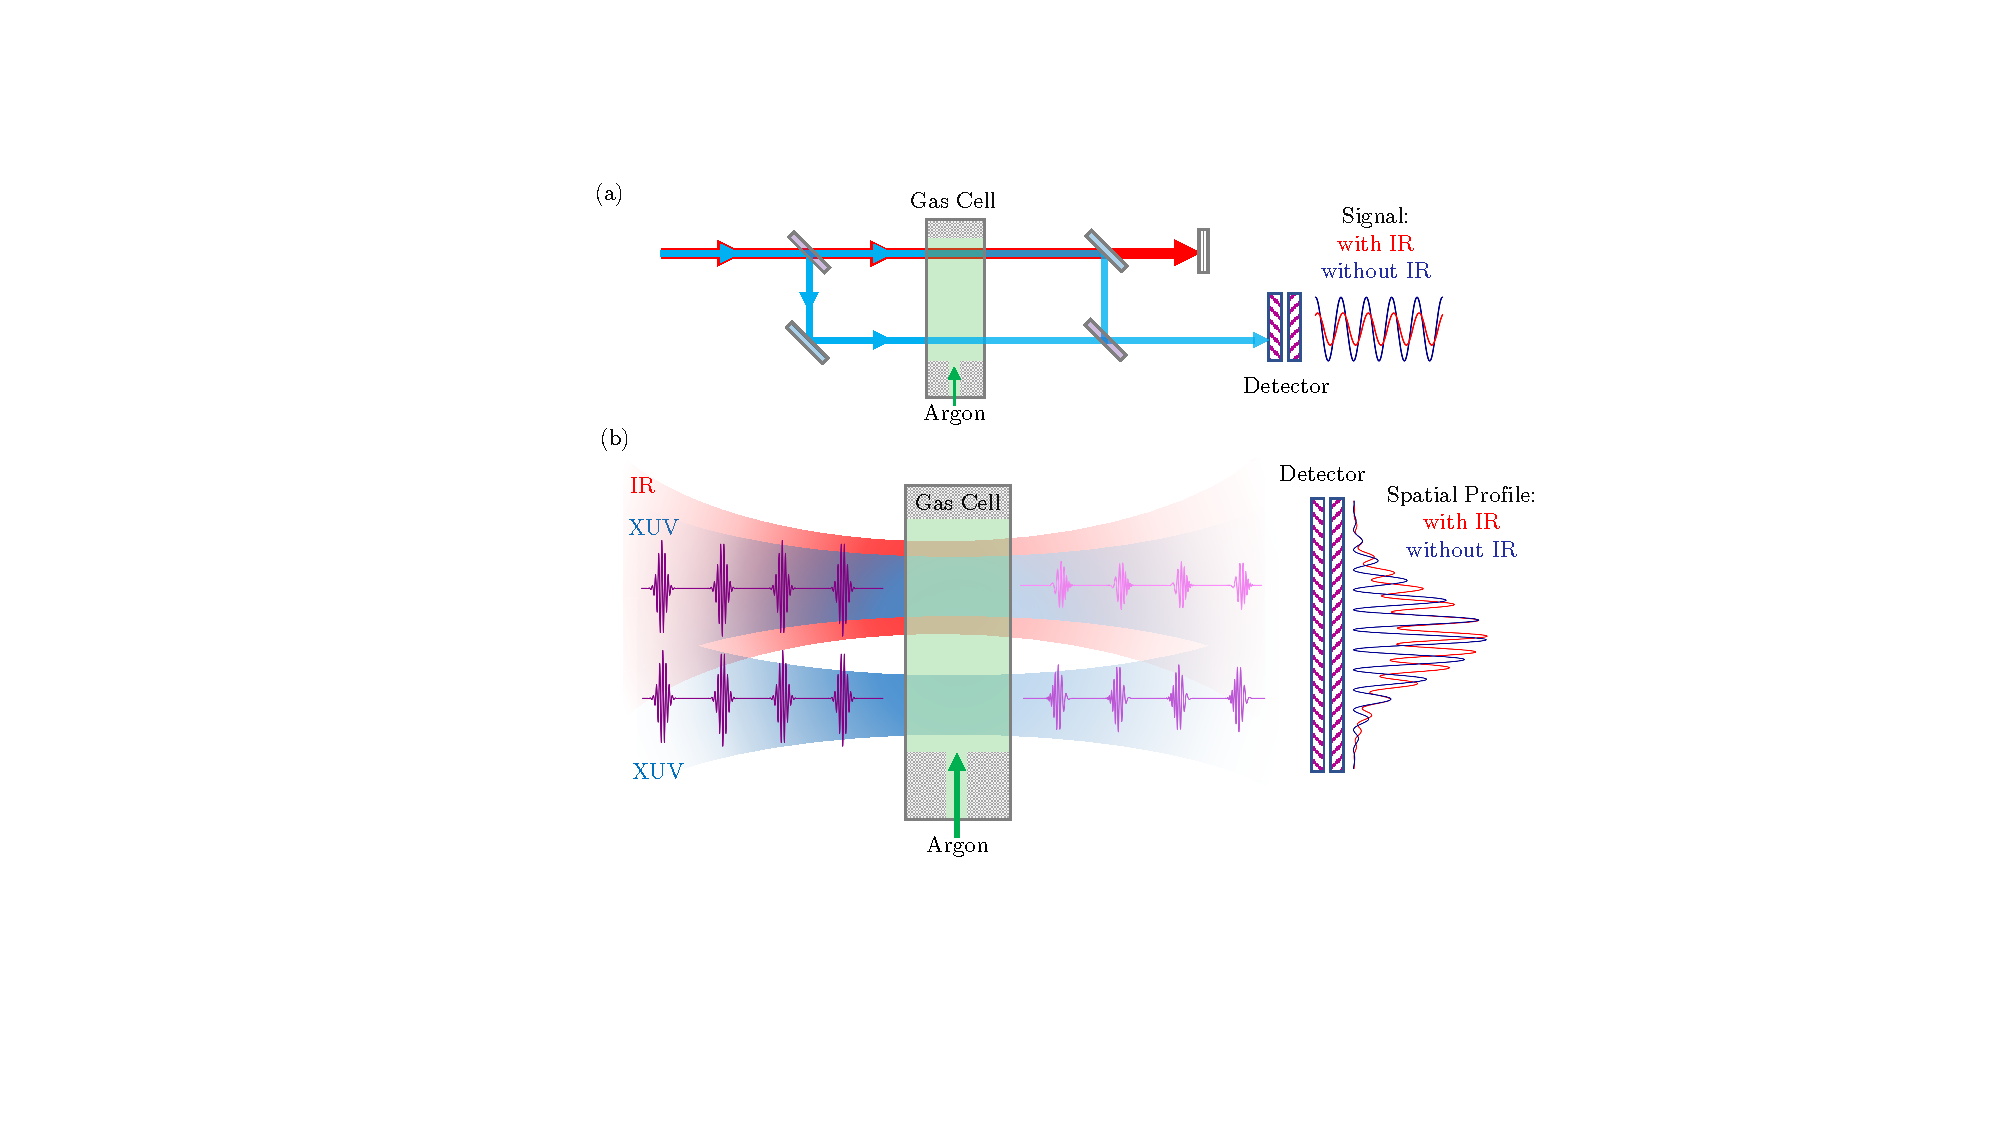
\includegraphics[width=1.0\textwidth]{figures/CATS/CATS_mach_zehnder.pdf}
	\caption[Schematic of Mach-Zehnder interferometer and spatial profile with and without an IR dressing field in one arm of the interferometer]{(a) Schematic of a Mach-Zehnder interferometer that is used to measure the phase shift induced by an IR dressing field introduced into one of the arms of the interferometer. (b) For the experiments described in this chapter, the two XUV sources will act as the two arms of a Mach-Zehnder, and the sample of interest will only be dressed in one the sources by an IR field.}
	\label{fig:CATS_mach-zehnder_interferometer}
\end{figure}

\begin{figure}
	\centering
	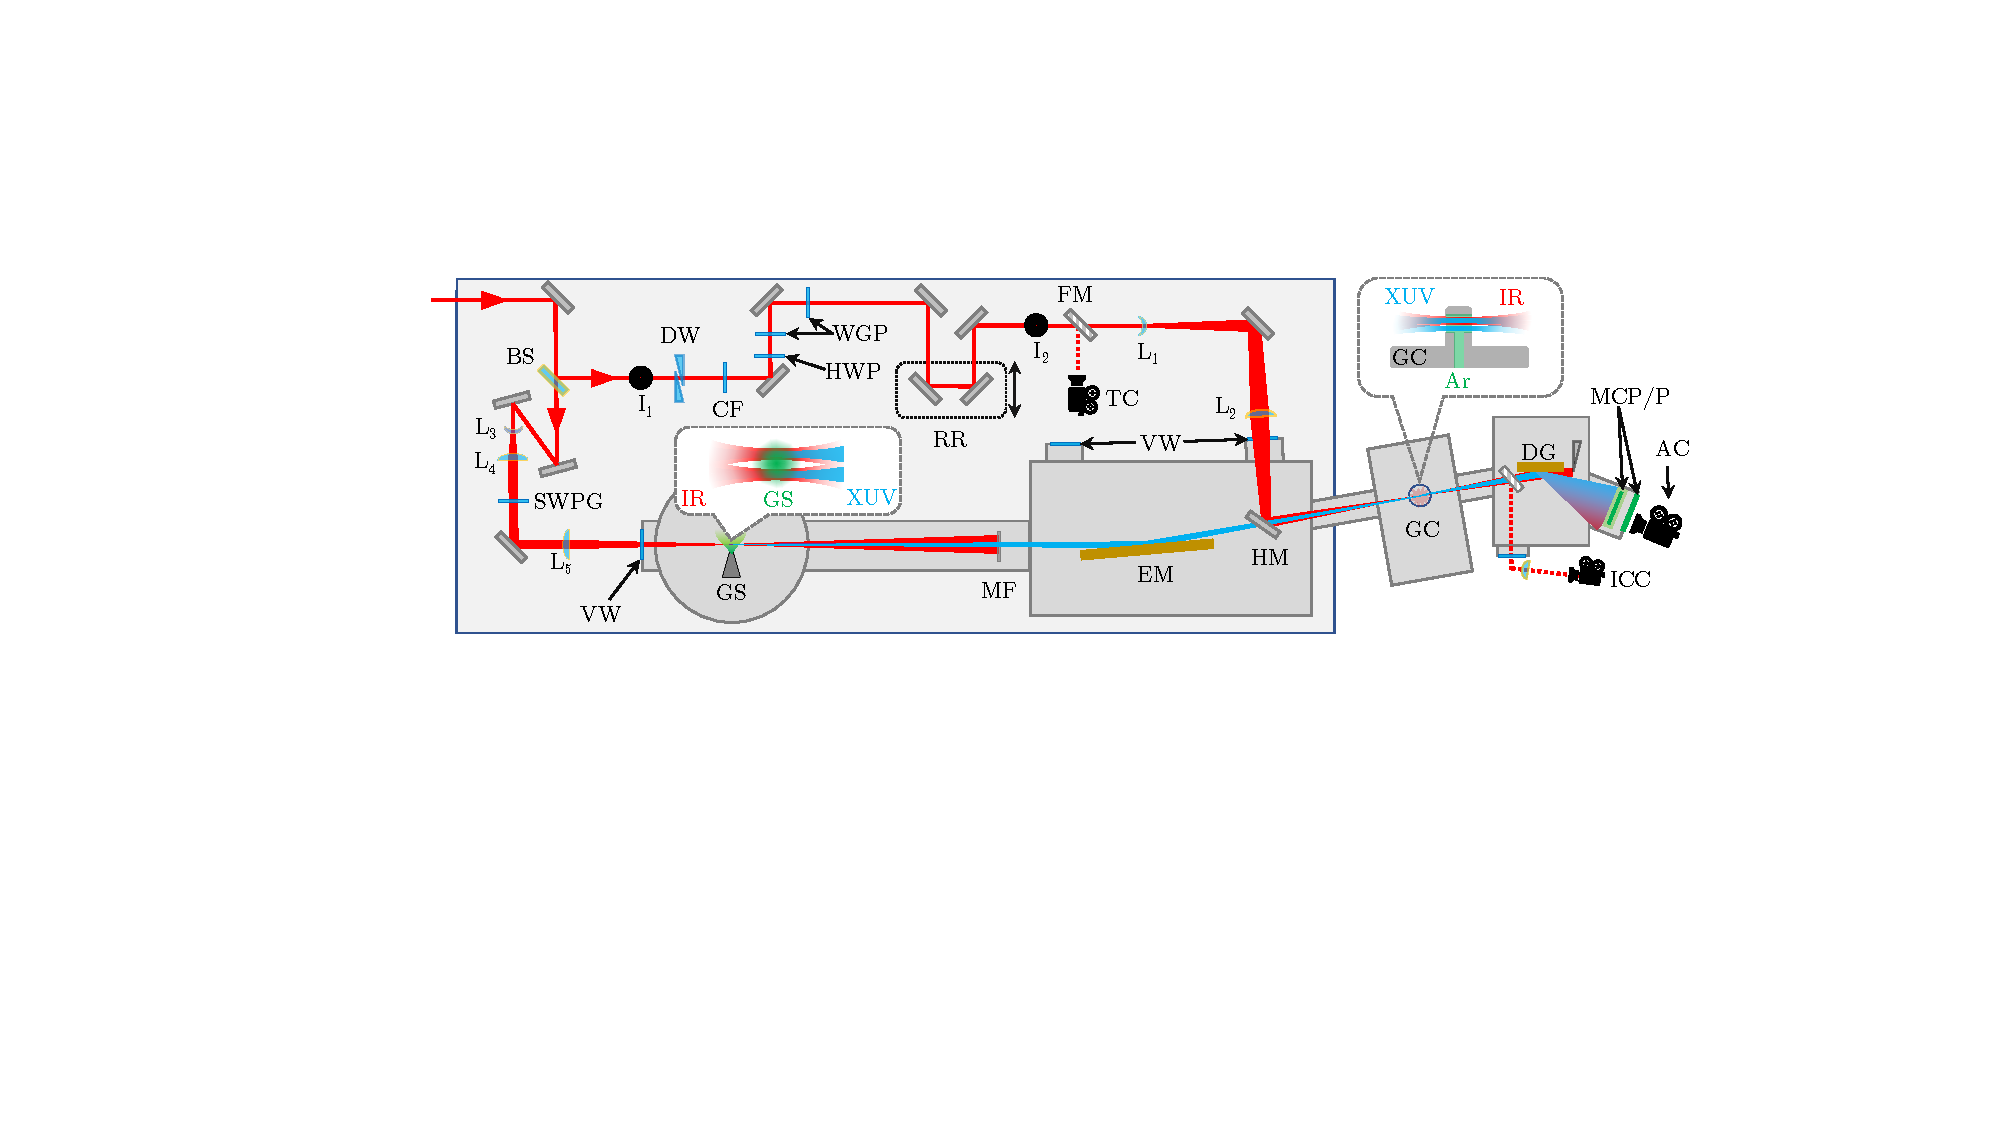
\includegraphics[width=1.0\textwidth]{figures/CATS/beamline_schematic_CATS.pdf}
	\caption[TABLe experimental setup for ATS experiments]{Schematic of the optical setup for the experiments described in this chapter.  \textbf{BS}: Beamsplitter (Thorlabs BSF20-C), \textbf{I$_{1,2}$}: Irises used for alignment. \textbf{DW}: Delay wedges for fine delay control. \textbf{CF}: Color filter (Thorlabs FELH1000). \textbf{HWP}: Half-wave plate. \textbf{WGP}: Wire grid polarizer. \textbf{RR}: Retro reflector for coarse delay adjustment.  \textbf{FM}: Flip mirror. \textbf{TC}: Thermal camera used for alignment.  \textbf{L$_1$}: $f=-300$ mm lens (Thorlabs LF1015-C). \textbf{L$_2$}: $f=500$ mm lens (Thorlabs LA1380-C). \textbf{VW}: Vacuum window, 3 mm CaF$_2$, \textbf{HM}: Hole mirror with 10 mm hole.  \textbf{L$_3$}: $f=-400$ mm lens.  \textbf{L$_4$}: $f=500$ mm lens. \textbf{L$_5$}: $f=400$ mm lens.  \textbf{BBO}: Second-harmonic generation crystal.  \textbf{Cal}: Calcite. \textbf{GS}: Gas source for HHG. \textbf{MF}: Aluminum filter. \textbf{EM}: Ellipsoidal mirror. \textbf{GC}: Gas cell. \textbf{RM}: Removable mirror for \textit{in-situ} diagnotics.    \textbf{ICC}: camera for \textit{in-situ} diagnotics. \textbf{DG}: VLS diffraction grating. \textbf{BB}: Baffles to block zero order diffraction.  \textbf{MCP/P}: Microchannel plate and phosphor.  \textbf{AC}: Andor Neo 5.5 CMOS camera.}
	\label{fig:CATS_setup}
\end{figure}

\section{Complex Attosecond Transient-absorption Spectroscopy of Fano resonances}
\label{sec:CATS_ar}

\subsection{Experimental setup}
\label{sec:CATS_ar_exp_setup}

\subsection{Results}
\label{sec:CATS_ar_results}


\section{Conclusion}
\label{sec:CATS_conclusion}